\section{Introduction}

\begin{frame}{The authors}
    \begin{columns}
        \begin{column}{0.5\textwidth}
            Jérémy Turi
            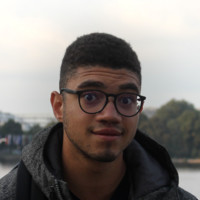
\includegraphics[width = 0.7\textwidth]{images/jeremy.jpeg}
            \begin{itemize}
                \item PhD Student at LAAS-CNRS
                \item Teacher at INSA Toulouse
            \end{itemize}
        \end{column}
        \begin{column}{0.5\textwidth}
            Dr. Arthur Bit-Monnot
            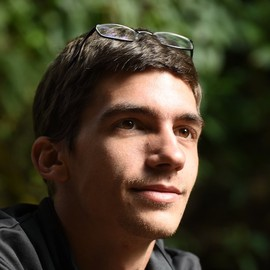
\includegraphics[width = 0.7\textwidth]{images/arthur.jpg}
            \begin{itemize}
                \item Researcher at LAAS-CNRS
                \item Associate Professor at INSA Toulouse
            \end{itemize}
        \end{column}
    \end{columns}
\centering    
\end{frame}

\begin{frame}{The research team}
\centering
    Robotics and Interactions (RIS) team:
    
    ~~

\begin{columns}
    \begin{column}{0.5\textwidth}
\begin{itemize}
    \item Human Robot Interaction
    \item Drones
    \item Deliberation algorithm: planning, acting, \dots
    \item Robotics architecture
\end{itemize}
    \end{column}
    \begin{column}{0.5\textwidth}
        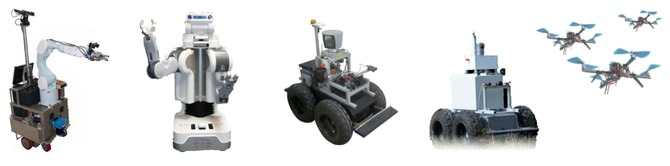
\includegraphics[width=\textwidth]{images/RIS-robot-banner.jpg}
    \end{column}
\end{columns}

\end{frame}
\begin{frame}{Scientific interests of the authors}
    \centering

\begin{itemize}
    \item Hierarchical and temporal planning
    \item Scalability of robotic architecture and deliberation algorithms.
\end{itemize}

~

My PhD Subject :

Planning from operational models for deliberative acting in robotics.

\end{frame}

\begin{frame}{The scope of the paper}
    Goal of the study: adapt a refinement acting engine (RAE) for multi-agents to
    \begin{itemize}
        \item Deal with concurrency
        \item Improve the interleaving of parallel tasks
        \item Reason on shared resources to optimize the overall process
    \end{itemize}
\end{frame}